% Options for packages loaded elsewhere
\PassOptionsToPackage{unicode}{hyperref}
\PassOptionsToPackage{hyphens}{url}
%
\documentclass[
]{article}
\usepackage{amsmath,amssymb}
\usepackage{iftex}
\ifPDFTeX
  \usepackage[T1]{fontenc}
  \usepackage[utf8]{inputenc}
  \usepackage{textcomp} % provide euro and other symbols
\else % if luatex or xetex
  \usepackage{unicode-math} % this also loads fontspec
  \defaultfontfeatures{Scale=MatchLowercase}
  \defaultfontfeatures[\rmfamily]{Ligatures=TeX,Scale=1}
\fi
\usepackage{lmodern}
\ifPDFTeX\else
  % xetex/luatex font selection
\fi
% Use upquote if available, for straight quotes in verbatim environments
\IfFileExists{upquote.sty}{\usepackage{upquote}}{}
\IfFileExists{microtype.sty}{% use microtype if available
  \usepackage[]{microtype}
  \UseMicrotypeSet[protrusion]{basicmath} % disable protrusion for tt fonts
}{}
\makeatletter
\@ifundefined{KOMAClassName}{% if non-KOMA class
  \IfFileExists{parskip.sty}{%
    \usepackage{parskip}
  }{% else
    \setlength{\parindent}{0pt}
    \setlength{\parskip}{6pt plus 2pt minus 1pt}}
}{% if KOMA class
  \KOMAoptions{parskip=half}}
\makeatother
\usepackage{xcolor}
\usepackage[margin=1in]{geometry}
\usepackage{longtable,booktabs,array}
\usepackage{calc} % for calculating minipage widths
% Correct order of tables after \paragraph or \subparagraph
\usepackage{etoolbox}
\makeatletter
\patchcmd\longtable{\par}{\if@noskipsec\mbox{}\fi\par}{}{}
\makeatother
% Allow footnotes in longtable head/foot
\IfFileExists{footnotehyper.sty}{\usepackage{footnotehyper}}{\usepackage{footnote}}
\makesavenoteenv{longtable}
\usepackage{graphicx}
\makeatletter
\def\maxwidth{\ifdim\Gin@nat@width>\linewidth\linewidth\else\Gin@nat@width\fi}
\def\maxheight{\ifdim\Gin@nat@height>\textheight\textheight\else\Gin@nat@height\fi}
\makeatother
% Scale images if necessary, so that they will not overflow the page
% margins by default, and it is still possible to overwrite the defaults
% using explicit options in \includegraphics[width, height, ...]{}
\setkeys{Gin}{width=\maxwidth,height=\maxheight,keepaspectratio}
% Set default figure placement to htbp
\makeatletter
\def\fps@figure{htbp}
\makeatother
\setlength{\emergencystretch}{3em} % prevent overfull lines
\providecommand{\tightlist}{%
  \setlength{\itemsep}{0pt}\setlength{\parskip}{0pt}}
\setcounter{secnumdepth}{5}
\newlength{\cslhangindent}
\setlength{\cslhangindent}{1.5em}
\newlength{\csllabelwidth}
\setlength{\csllabelwidth}{3em}
\newlength{\cslentryspacingunit} % times entry-spacing
\setlength{\cslentryspacingunit}{\parskip}
\newenvironment{CSLReferences}[2] % #1 hanging-ident, #2 entry spacing
 {% don't indent paragraphs
  \setlength{\parindent}{0pt}
  % turn on hanging indent if param 1 is 1
  \ifodd #1
  \let\oldpar\par
  \def\par{\hangindent=\cslhangindent\oldpar}
  \fi
  % set entry spacing
  \setlength{\parskip}{#2\cslentryspacingunit}
 }%
 {}
\usepackage{calc}
\newcommand{\CSLBlock}[1]{#1\hfill\break}
\newcommand{\CSLLeftMargin}[1]{\parbox[t]{\csllabelwidth}{#1}}
\newcommand{\CSLRightInline}[1]{\parbox[t]{\linewidth - \csllabelwidth}{#1}\break}
\newcommand{\CSLIndent}[1]{\hspace{\cslhangindent}#1}
\ifLuaTeX
  \usepackage{selnolig}  % disable illegal ligatures
\fi
\IfFileExists{bookmark.sty}{\usepackage{bookmark}}{\usepackage{hyperref}}
\IfFileExists{xurl.sty}{\usepackage{xurl}}{} % add URL line breaks if available
\urlstyle{same}
\hypersetup{
  pdftitle={Lessons learned: creating tutorials teaching Agent-Based Modelling for Archaeologists},
  hidelinks,
  pdfcreator={LaTeX via pandoc}}

\title{Lessons learned: creating tutorials teaching Agent-Based Modelling for Archaeologists}
\author{true \and true \and true \and true \and true \and true \and true \and true \and true \and true}
\date{September 20, 2024}

\begin{document}
\maketitle

{
\setcounter{tocdepth}{2}
\tableofcontents
}
\hypertarget{introduction}{%
\section{Introduction}\label{introduction}}

Computational modelling has become a standard research technique across most scientific disciplines, including archaeology. Among the many computational modelling techniques the discipline has found agent-based modelling to be particularly well suited to the questions asked by archaeologists. Agent-based modelling is a simulation technique where autonomous agents interact with each other and with their environment. Their aggregated behaviour gives rise to system-level outcomes thus enabling researchers to understand how \emph{micro} (individual) \emph{mechanisms} lead to \emph{macro} (system-level) \emph{patterns}.

While Agent-Based Modelling importance in archaeological practice is steadily growing (Romanowska and Scherjon 2023) there are significant bariers to its wider adoption. One of the sectorial problems is the access to vocational training required to gain the necessary computer programming and modelling skills. A survey of practitioners (Davies and Romanowska 2018) found significant deficiencies in the provision of ABM training; 76\% of modellers were primarily self-taught with some degree of secondary support i.e.~27\% relied on peer support, only 7\% had any sort of formal training at a workshop or summer school, while only 14\% received training as part of a degree.

A consortium of Landward Research Teoranta, Aarhus Universitet, Universiteit Leiden and Saxion University of Applied Sciences recognised this need, and sought to address the limited opportunities that archaeologists have to access high quality training through a project aiming to create and make available open learning materials that could be integrated into a wide range of training programmes, such as face-to-face training, employer-focussed continuing professional development seminars, webinars, MOOCs (Massive Open Online Courses) and self-directed learning.

This project, Agent-Based Modelling for Archaeologists, was delivered with the support of the Erasmus+ programme of the European Union.

The project sought to create Open (Open Access and Open Source) Educational Resources (OERs) for training in Agent-Based Modelling for Archaeologists. These OERs were to be HTML and JavaScript based so they could be used on any device with a browser, even if it is not connected to the internet. The full programme consists of five hands-on practical tutorials, taking learners through the process of creating the digital models. The modular architecture ensures that they can be independent or incorporated into other teaching tools like learning management systems. They are also deliberately `method agnostic' so they can be incorporated into any tools from self-teaching to MOOCs, and are supported by a set of support materials to encourage use of the OERs.

The activities the project implemented were:

\begin{itemize}
\item
  development of a hands-on vocational training programme, aligned with the recently published \emph{Agent-Based Modelling for Archaeology: Simulating the Complexity of Societies} (Romanowska, Wren and Crabtree 2021);
\item
  conversion of the training programme into modular learning resources that are interactive, based on HTML and JavaScript standards;
\item
  creation of support materials to encourage use of the OERs;
\item
  creation of how-to guides to help trainers incorporate OERs into their teaching;
\item
  creation of a code and learning materials repository that will allow the project to continue sustainability after the European Union support has ended and to facilitate the creation of an open-source community to manage and improve the OERs in the future;
\item
  development of the framework for skills acquisition aligned with the Digital Skills Passport;
\item
  promotion through a series of multiplier events.
\end{itemize}

The expected results and outcomes, for the target audience of professional archaeologists, were:

\begin{enumerate}
\def\labelenumi{\arabic{enumi}.}
\item
  a surge in professionals who can build, apply and critique archaeological simulation thus opening new research avenues for the discipline as a whole;
\item
  increased level of digital competence, specifically in advanced computer skills that are highly transferable to other industries. This includes technical skills such as programming but also ``soft'' skills related to computational thinking;
\item
  improved opportunities for archaeologists to work in other European countries (transnational mobility) through matching the skills being delivered with the European Commission's Digital Competence Framework for Citizens (2.2) and the sectoral Skills Passport for Archaeology, which will mean that it will be easier for individual workers to demonstrate their skills to employers across Europe;
\item
  increased opportunities for professional development by having access to professional training that can be incorporated into formal or non-formal/informal learning.
\end{enumerate}

For the secondary target audience of vocational training providers in archaeology e.g.~employers, colleges and not-for-profit organisations, the expected results and outcomes were:

\begin{enumerate}
\def\labelenumi{\arabic{enumi}.}
\item
  increased quality of training in Agent-based Modelling that is free and open;
\item
  access to teaching materials for skills that are in high demand and aligned with employers' needs.
\end{enumerate}

We were able to draw on previous experiences with a small private online course (SPOC) on `Modelling and Simulation in Archaeology' that some of us designed for graduate teaching at the Faculty of Archaeology, Leiden University, where we taught this course in 2016/17 and again in 2018/19 (Scherjon, Romanowska and Lambers 2019). For this course we developed new online teaching materials comprising pre-recorded lectures, practical exercises, reading assignments and exams. While we greatly benefited from that experience, the target group of the SPOC was graduate students with prior experience in digital archaeology, whereas the ERASMUS+ project was aimed at a much broader target group of archaeology students and professionals whose computational literacy could not be assumed.

\hypertarget{method}{%
\section{Method}\label{method}}

The project team developed five online tutorials. The tutorials were first designed using storyboards and later converted into interactive guided walk-throughs using NetLOGO Web (\url{https://www.netlogoweb.org/launch}) and Javascript and hosted on GitHub (\url{https://github.com/ABMArchaeologists/ABMA_tutorials}). During the project, initial testing was done by all authors and issues in GitHub were used to tackle bugs.

The ABMA learning materials assume that participants have learning skills at least at a secondary education level. It is suitable for participants with at least some background in archaeology, such as those typical among students after the first year of a Bachelor study in Archaeology, i.e., above EQF levels 4 or 5. In addition, the tutorials are aimed at professionals working in archaeology who have some experience with computer applications. We also assume that learners are proficient in English and have at least the Reading B1 level, but Reading B2 is recommended (Council of Europe 2020). The tutorials were also developed with a secondary aim to develop learners' general skills in the following competence area's: 1. Information and data literacy, 2. Communication and collaboration, 3. Digital content creation and, 5. Problem solving (European Commission, Joint Research Centre et al. 2022).

After initial debugging by the project team, the tutorials were tested on a wider sample of participants during several online and in-person events all of which were run by members of the project team. Recognising the difficulty of delivering practical training in an online environment during the online events several members of the team were present which enabled participants to go to break-out rooms with an expert if they needed additional help or wanted to discuss things. Throughout the project we sought feedback from the participants and used it to improve the tutorials prior to the following events. The feedback was obtained through two surveys using Qualtrics (\url{https://www.qualtrics.com/}). The participants of the events were asked to respond to two surveys: one before the start of the event and one completed after the end of the event. The first survey focused on the background of the participants and their original level of knowledge in relation to ABM (see appendix 1 for the questions). At the end of the event the participants were asked to answer a second survey. Questions of this survey were aimed at measuring the effectiveness of the tutorials and getting feedback on the workshop and tutorials (see appendix 2 for the questions). For some events participants had to register beforehand and we were able to send the pre-workshop survey by email. At other events no registration was possible or necessary and the pre-workshop survey was given at the start of the event. The post-workshop survey was distributed using QR-codes or links at the end of the event.

\begin{longtable}[]{@{}
  >{\raggedright\arraybackslash}p{(\columnwidth - 8\tabcolsep) * \real{0.2256}}
  >{\raggedright\arraybackslash}p{(\columnwidth - 8\tabcolsep) * \real{0.1880}}
  >{\raggedright\arraybackslash}p{(\columnwidth - 8\tabcolsep) * \real{0.2180}}
  >{\raggedright\arraybackslash}p{(\columnwidth - 8\tabcolsep) * \real{0.1805}}
  >{\raggedright\arraybackslash}p{(\columnwidth - 8\tabcolsep) * \real{0.1880}}@{}}
\caption{Conferences, events and situations were workshops were held at which the tutorials were tested.}\tabularnewline
\toprule\noalign{}
\begin{minipage}[b]{\linewidth}\raggedright
Conference or event
\end{minipage} & \begin{minipage}[b]{\linewidth}\raggedright
Period
\end{minipage} & \begin{minipage}[b]{\linewidth}\raggedright
Online, in person or hybrid
\end{minipage} & \begin{minipage}[b]{\linewidth}\raggedright
Number of participants
\end{minipage} & \begin{minipage}[b]{\linewidth}\raggedright
Number of registrations
\end{minipage} \\
\midrule\noalign{}
\endfirsthead
\toprule\noalign{}
\begin{minipage}[b]{\linewidth}\raggedright
Conference or event
\end{minipage} & \begin{minipage}[b]{\linewidth}\raggedright
Period
\end{minipage} & \begin{minipage}[b]{\linewidth}\raggedright
Online, in person or hybrid
\end{minipage} & \begin{minipage}[b]{\linewidth}\raggedright
Number of participants
\end{minipage} & \begin{minipage}[b]{\linewidth}\raggedright
Number of registrations
\end{minipage} \\
\midrule\noalign{}
\endhead
\bottomrule\noalign{}
\endlastfoot
CAA Amsterdam & April 2023 & In person & 36 & 53 \\
EAA Belfast & August 2023 & In person & 21 & No registration \\
CAA-DE/NL-Fl Online workshop & October 2023 & Online & 40 & 76 \\
Reuvensdagen & November 2023 & In person & 13 & No registration \\
CAA-UK & November 2023 & Hybrid & 53 & No registration \\
Leiden (course) & December 2023 & In person & 11 & No registration \\
Aarhus & January/February 2024 & Online & 176 & \textgreater500 \\
Saxion & March 2023-January 2024 & In person & 18 & No registration \\
\textbf{Total} & & & \textbf{368} & \textbf{\textgreater628} \\
\end{longtable}

The surveys were analysed using R (R Core Team 2023). The following packages were used for analyses: ggplot2 (Wickham 2016), dplyr (Wickham et al. 2023), tidyr (Wickham, Vaughan and Girlich 2023), forcats(Wickham 2023a), lubridate (Grolemund and Wickham 2011) and stringr (Wickham 2023b). For the sake of reproducibility (Marwick 2017) this paper was written in R Markdown (\url{https://rmarkdown.rstudio.com/}), with data and code available at \url{https://github.com/ABMArchaeologists/ABMA_paper} (\ldots{} insert Zenodo reference\ldots)

Over the course of the project three groups of students worked on the project during the Smart Solutions Semester at Saxion University of Applied Sciences. This is an interdisciplinary semester in which students of at least three different study-programmes or disciplines work together on a complex problem/project (\url{https://www.saxion.edu/business-and-research/collaborate-with-saxion/smart-solutions}). Within the semester students have to come up with new ideas or solutions to help a client with a wicked problem. The backgrounds of the various students we worked with were diverse: Applied Computer Science, Archaeology, Business Management Studies, Creative Business, Creative Media \& Game Technologies, and ICT. The aim of involving interdisciplinary groups in the project was to involve students in current research projects, to enable them to learn new things and share their innovative ideas and solutions with us. The students groups were supplementary to the deliverables of the project, but their new ideas were benificial to the project. Their help during workshops was useful, but they also were engaged in developing educational material (Aalpoel et al. 2024), testing the tutorials, developing a style for the website (Jutte et al. 2024) and other materials.

\hypertarget{results}{%
\section{Results}\label{results}}

\hypertarget{workhops-and-tutorials}{%
\subsection{Workhops and tutorials}\label{workhops-and-tutorials}}

\hypertarget{final-tutorials}{%
\subsection{Final tutorials}\label{final-tutorials}}

The final set of ABMA tutorals are available for download at \url{https://github.com/ABMArchaeologists/ABMA_tutorials} and are citeable (Rocks-Macqueen et al. 2024). The set of developed tutorials consists of the following tutorials:

\begin{itemize}
\item
  Tutorial 1: Introduction to ABM
\item
  Tutorial 2: Beginning with NetLogo
\item
  Tutorial 3: Expanded ABM skills
\item
  Tutorial 4: Intermediate ABM
\item
  Tutorial 5: How to Model
\end{itemize}

Each tutorials consists of a number of individual lessons, each of which guides the learner in a self-pace manner through an increasingly challenging set of exercises that build the skills and knowledge necessary to become a confident agent-based modeller.

In the first tutorial the user learn what simulations and agent-based models are and how they can help in archaeological research. This tutorial consists of 4 lessons. The first two lessons introduce the learner to simulation in general and Agent-Based Modelling in specific. Various concepts related to ABM, such as the definitions of model and simulation, are introduced and the participants make their first steps in NetLogo syntax. The third lesson explains how ABMs are used in archaeological research. The final lesson introduces the learner to the NetLogo Interface and the difference between the Interactive and Authoring mode. This tutorial builds a foundation for working in NetLogo and with ABM. All activity stays within the entree level of difficulty, although some higher level concepts are lightly touched upon.

\begin{figure}
\centering
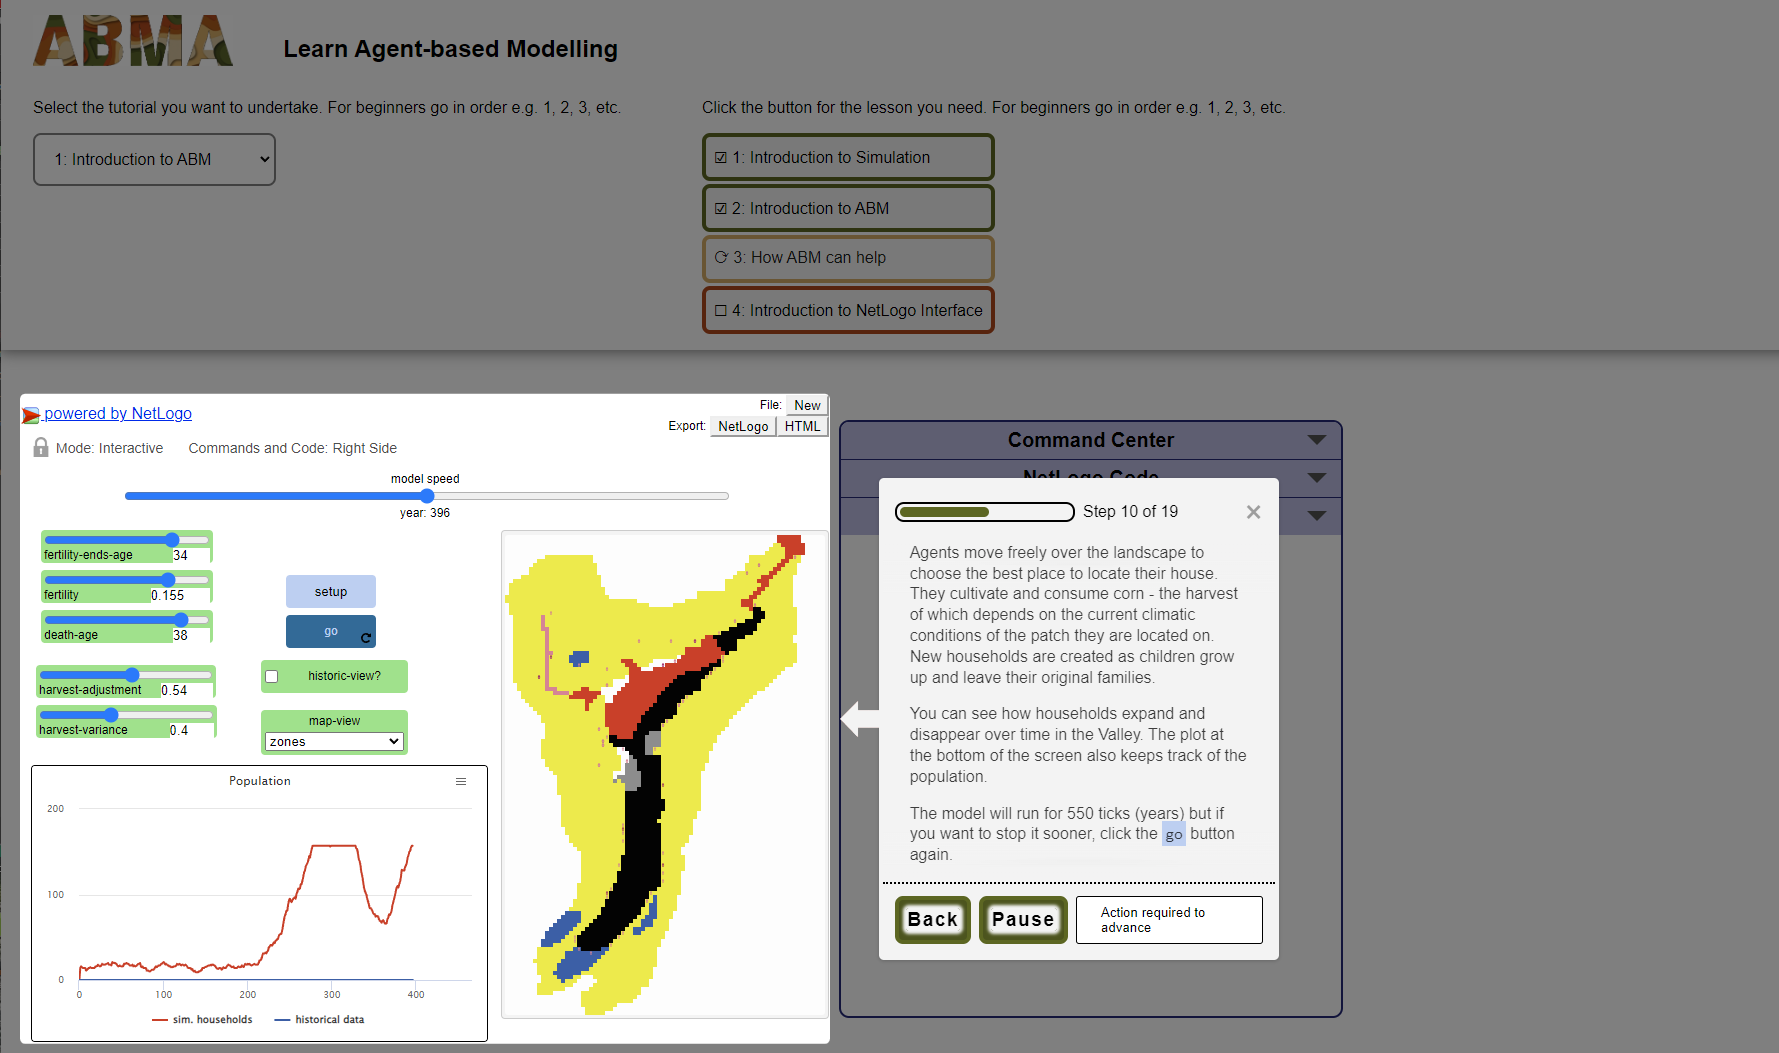
\includegraphics{paper_files/Screenshot_ABMA_tutorial_1_lesson_3.png}
\caption{Screenhot of lesson 3 in tutorial 1 showing the population dynamics of the Long House Valley in the Artificial Anasazi model created by Axtell et al.~(2002).}
\end{figure}

In tutorial 2 the user will learn the basics of NetLogo by making your their simulation on the Out of Africal dispersal of \emph{Homo sapiens} (Young and Bettinger 1995).The learner works through the basics of NetLogo syntax and learn how to set up a simulation and visualize its outcomes. This tutorial consists of 9 lessons. This tutorial intends to guide the learner from the introduction to the beginner level of proficiency. The learning curve is relatively gentle. This is achieved by working with the NetLogo web interface that enables highlighting specific words and buttons and giving visual cues as to how to proceed. The tutorial intoduces several most commonly used built-in functions in Netlogo (called \emph{primitives}) are introduces the general structure of all models cosisting of the initialization phase and the main simulation loop. It walks the participants through te most important NetLogo settings, such as dimensions, coordinates and the origin point of the grid on which the simulation runs. The learners gain their first stripes in programming by using simple loops and functions as well as conditional statements. The next level is achieved by introducing the topic of function definition and different types of variables. Exporting data produced by the model through plots is also explained.

In the third tutorial, the learner builds a simple trade model, again based on a published simulation (Romanowska 2018). Here learners are expanding their NetLogo programming skills with more complexity added to such syntactic structures as loops, lists and reporters. The learner is introduced to some key computational techniques like modular code development and debugging which become important alongside this increased coding complexity. This tutorial consists of 7 lessons. This tutorial intends to guide the learner from the beginner to the intermediate level of proficiency. This is achieved by introducing standards of code development such as modular code, pseudocode, debugging and annotating the code. In addition, the tutorial introduces custom agent breeds, visualization with labels and reporters, plots and monitors. This takes the learner to a more advanced level, since it develops knowledge of the programming language combined with diagnosing unexpected behaviour and problem solving.

In tutorial 4 the learner works with a seminal Sugarscape model (Epstein and Axtell 1996) to further expand their agent-based modelling and NetLogo skills. The learner explores how to set up more complex interactions between agents and the environment. Furthermore, the principles of setting up good experiments and validating models is explained. This tutorial consists of 8 lessons. This tutorial intends to solidify the learner's understanding at the intermediate level of proficiency by introducing yet more complex agent-environment interaction, alternative ways to visualize the environment and modelling spatial dynamics. Creating toy landscapes is central to lesson 5. The learner dives into the topic of experiment design at a practical level but also with regards to the scientific principles, such as validation. Thus they are guided through the process of setting up experiments in NetLogo and collecting results using monitors and plots. The topic of validation of agent-based models is critical for most archaelogical applications and thus several ways to compare simulation results with the archaeological record are explored.

In the final and fifth tutorial the participant learn smore about how to incorporate agent-based modelling in archaeological research. This tutorial focuses less on programming in NetLogo and more on the principle and standards of computer-based modelling. The learner learns about the different phases of the model development process. This tutorial consists of 5 lessons. This tutorial summarizes the material delivered in the previous lessons into one coherent framework consistent with an intermediate level of proficiency. This tutorial approaches more theoretical aspects in a practical environment. The learner revisits all phases of the model development process starting with the conceptual phase and finishing with the analysis and interpretation of results. There is a particular focus on discussing what kind of research questions are suitable for modelling and how to pick the right modelling technique. The importance of properly conceptualizing a model before starting the technical phase of the model development is highlighted as it is a common issue for less experienced modellers. The experiment design phase, including parametrisation, validation and the analysis and interpretation of the models is explained at length since it often prove challenging for students. On a practical side, the BehaviorSpace - NetLogo's experiment environment - is explained to enable the learners to batch run their models. Finally the dissemination phase of the model development is also included to ensure that the standards in model publication are widely known. Finally, the learners explores the fundamental importance of replication for advancing scientific knowledge.

\hypertarget{before-the-workshops}{%
\subsection{Before the workshops}\label{before-the-workshops}}

A large proportion of the participants of the workshops gave us information using the survey before the workshops (172 of 368 participants). The respondents came from at least 40 countries that represented almost all continents (see Figure \ref{fig:nationality}. There was a clear skew towards participants from Europe. The number of female respondents slightly outnumbers the male ones and a small group did not share their gender, while two identified as non-binary (see Figure \ref{fig:gender-age}). The ages of the respondents ranged from below 20 to over 70, although the majority fell between 20 and 40 years old indicating that the audience was predominantly composed of early career archaeologists. It seems that the different events also had a slightly different distribution of both gender and age. For example, more older people attended the workshop at the CAA conference in April 2023 and more men were present during the workshop at the Reuvensdagen in November 2023. This might be due the the differences of audiences at the conferences. For the Reuvensdagen the number of participants of the workshop was relatively low and this variance might be due to chance.

\begin{figure}
\centering
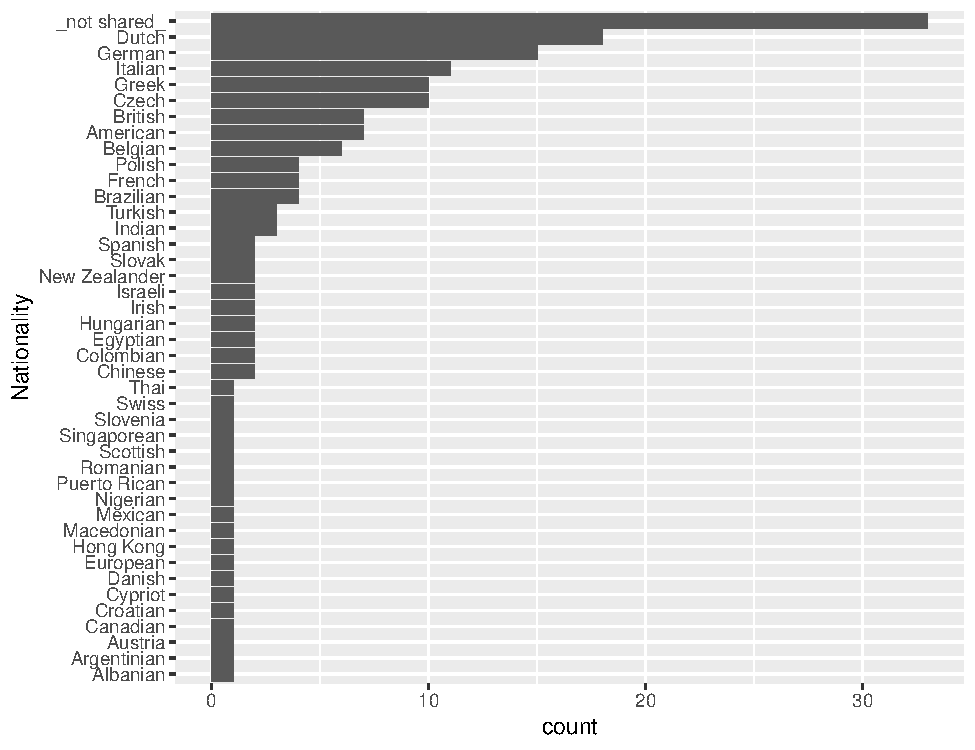
\includegraphics{paper_files/figure-latex/nationality-1.pdf}
\caption{\label{fig:nationality}The nationality of the participants that filled in the survey.}
\end{figure}

\begin{figure}
\centering
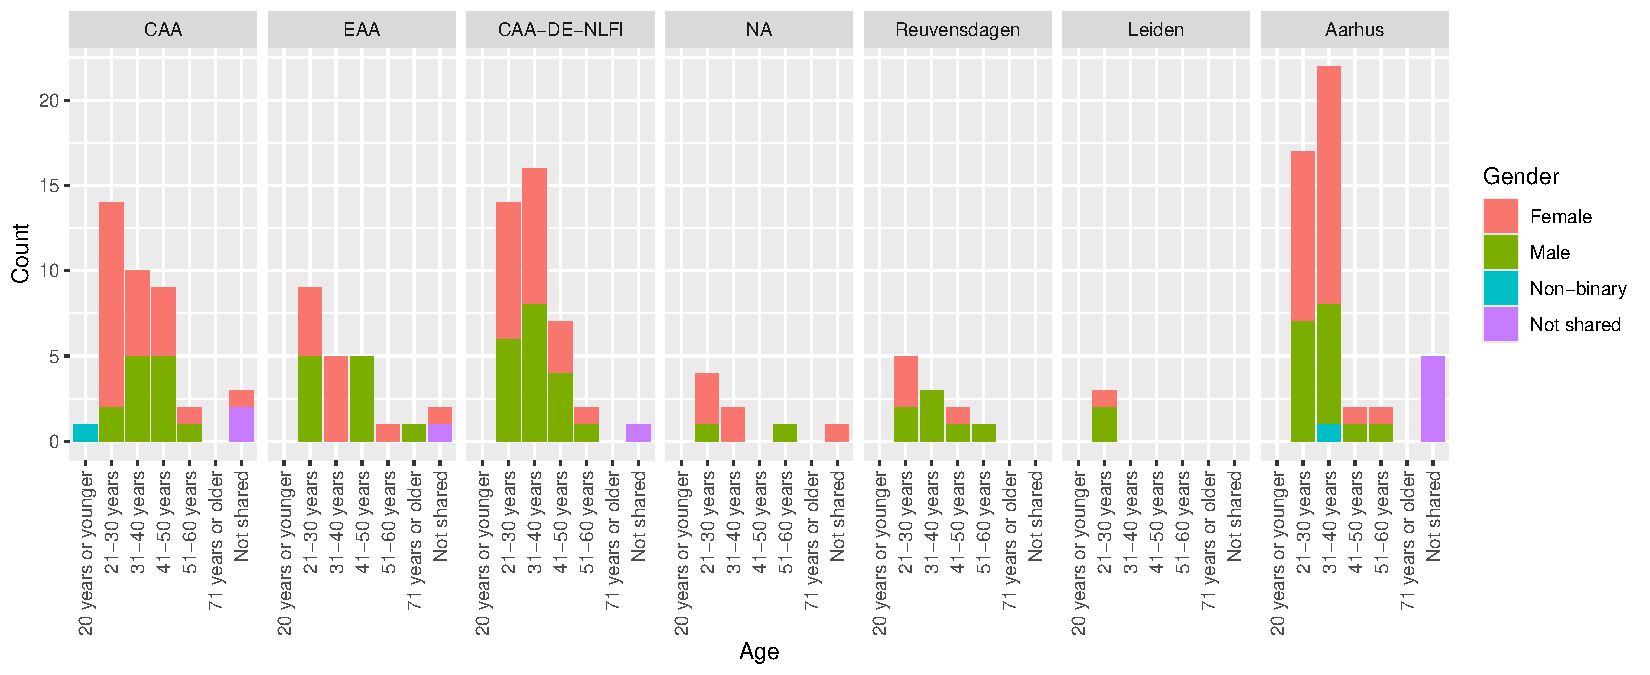
\includegraphics{paper_files/figure-latex/gender-age-1.pdf}
\caption{\label{fig:gender-age}The gender and age distribution of the respondents for each workshop}
\end{figure}

Most of the respondents reported having a level of computer literacy already including particular computational skills common in archaeology, for example working with word processors, GIS and spreadsheets (see Figure \ref{fig:computer-skills}), and 111 of the respondents had some prior knowledge of ABM, while 59 were completely new to the subject. The majority (158) had never applied ABM to their research before participating in the workshops with only 14 participants who had experience of developing archaeological ABM. It is interesting to note that many respondents (108) did know what kind of software was available for ABM (see Figure \ref{fig:abm-knowledge}).

\begin{figure}
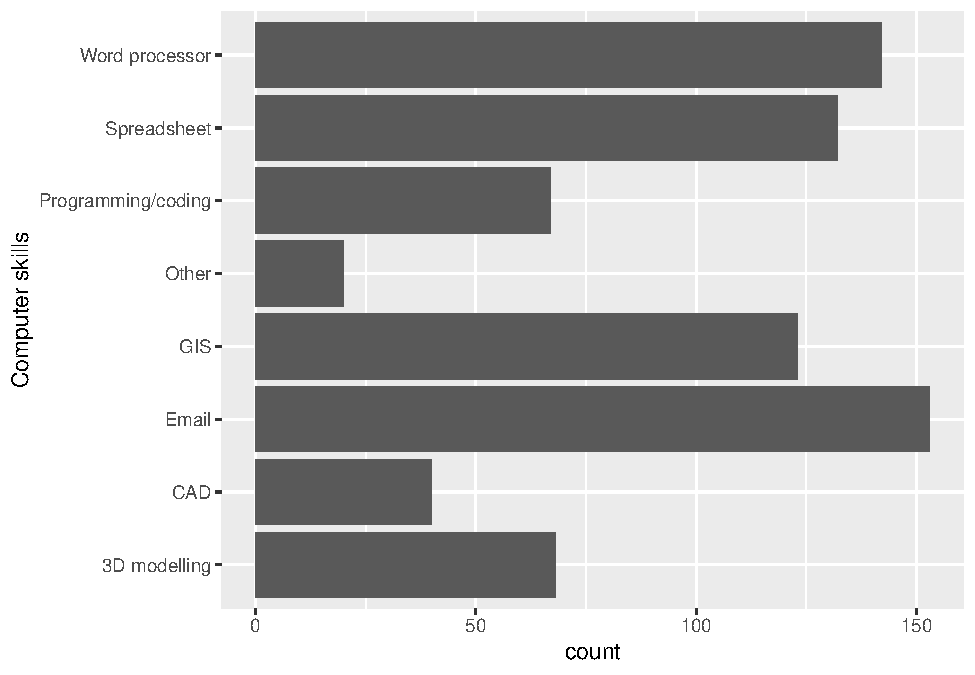
\includegraphics[width=0.5\linewidth]{paper_files/figure-latex/computer-skills-1} \caption{The computer skills of the respondents.}\label{fig:computer-skills}
\end{figure}

\begin{figure}
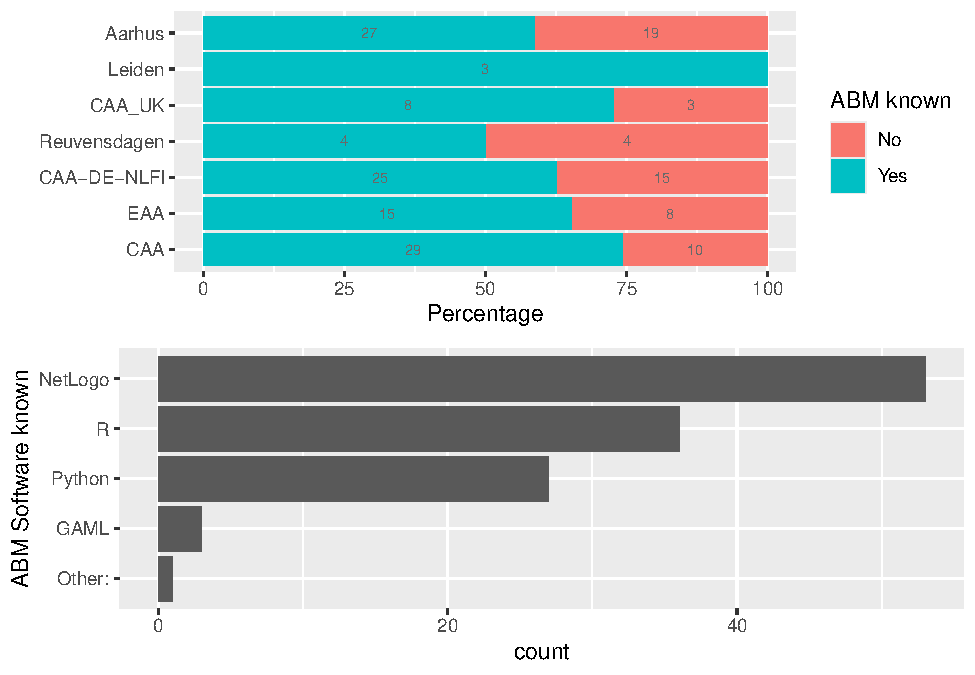
\includegraphics[width=0.5\linewidth]{paper_files/figure-latex/abm-knowledge-1} 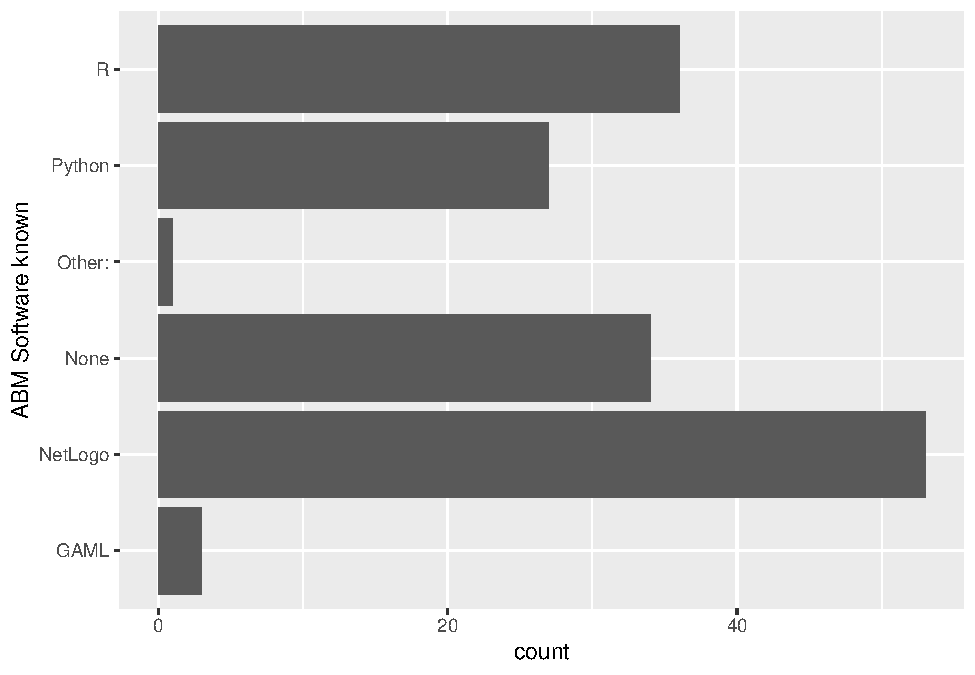
\includegraphics[width=0.5\linewidth]{paper_files/figure-latex/abm-knowledge-2} \caption{Respondents knowledge of ABM per event knowledge of the various softwares for ABM, before participating in the workshops.}\label{fig:abm-knowledge}
\end{figure}

As shown above, the respondents had some knowledge on ABM in general, but did not know how to apply it or had never applied it before. The respondents were also asked how they rated the available knowledge on ABM (Figure \ref{fig:available-theory}). While 64 of them had no opinion on the subject, a proportion of the respondents (28) answered that they rated the available theory on ABM as limited and only a small group (39) as sufficient or better. This clearly shows the need for more and better educational material.

\begin{figure}
\centering
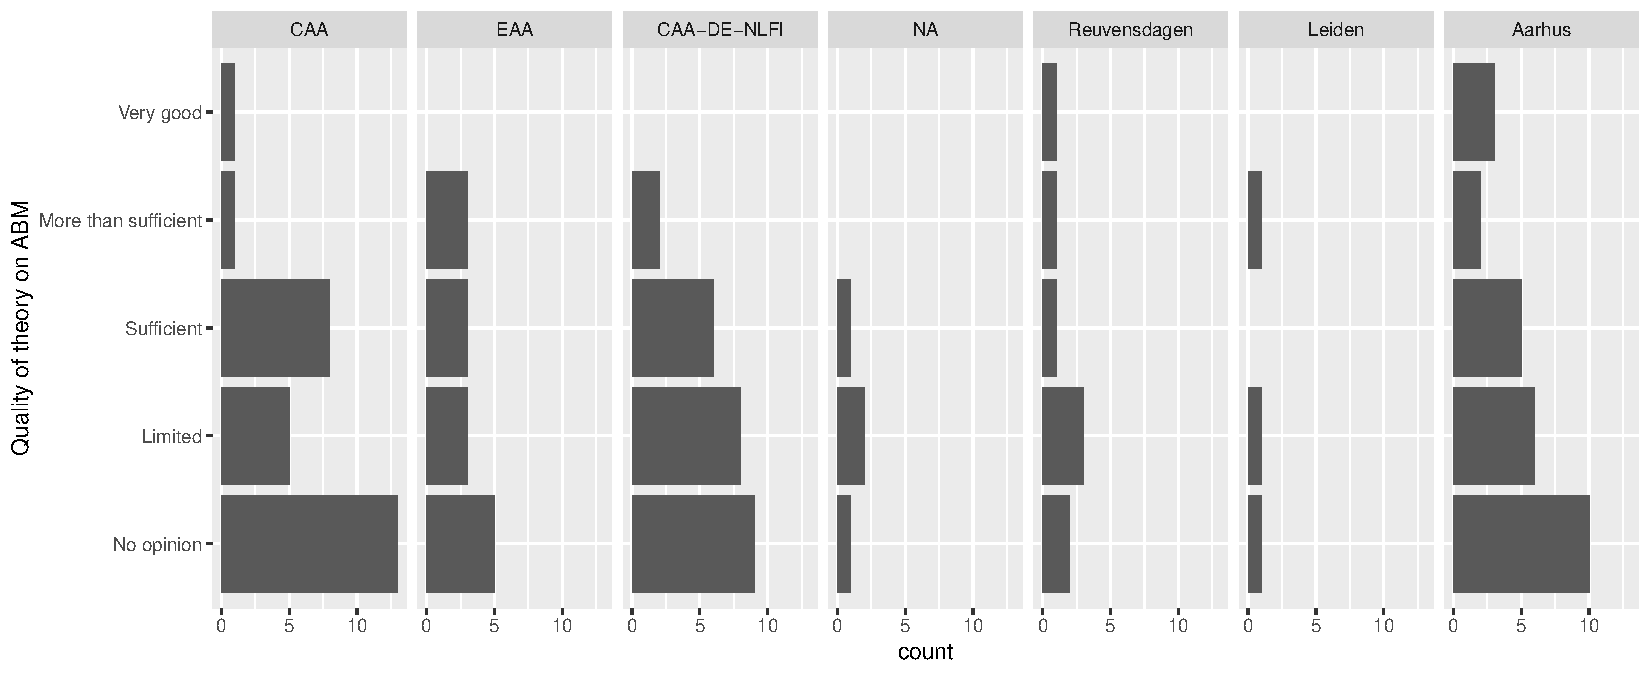
\includegraphics{paper_files/figure-latex/available-theory-1.pdf}
\caption{\label{fig:available-theory}Respondents optionion on the quality of theory on ABM faceted out by event.}
\end{figure}

\hypertarget{during-the-workshop}{%
\subsection{During the workshop}\label{during-the-workshop}}

During the workshops the participants worked in a self-paced manner, often on their own, but sometimes working together and discussing the tutorials. Some participants engaged in discussion with the teachers to learn how they could apply ABM in their research of discuss possibilities for the application of ABM in general. Individual progress varied depending on skills and preferences of the participants. While bugs were still a problem in earlier workshops, participant-teacher interaction was more focused on content-related learning problems in later installments.

\hypertarget{after-the-workshop}{%
\subsection{After the workshop}\label{after-the-workshop}}

A similar proportion of the participants of the workshops gave us information after the workshops (171 of 368 participants).

\begin{figure}
\centering
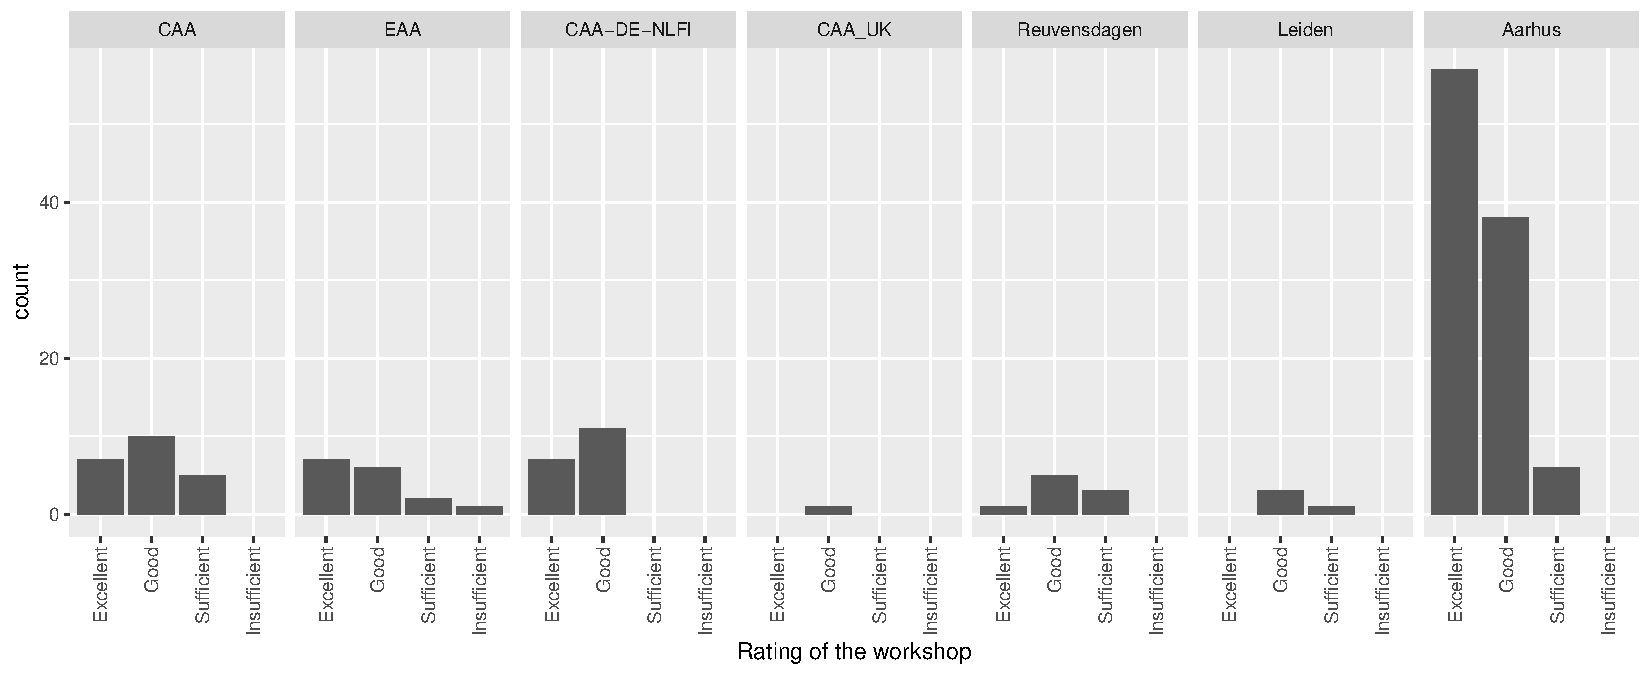
\includegraphics{paper_files/figure-latex/rating-workshop-1.pdf}
\caption{\label{fig:rating-workshop}Respondents rating of the workshop in general faceted for each event.}
\end{figure}

of the respondents were enthusiastic about the teaching material, with the majority rating it as excellent or good. The teachers were rated even higher than the teaching material, with more respondents giving them the \emph{excellent} score (see Figure \ref{fig:rating-teaching}).

The majority of the respondents (153) were enthusiastic about the teaching material, with the majority rating it as excellent or good. The teachers were even rated better than the teaching material, with more respondents (165) giving them the \emph{excellent} score (see Figure \ref{fig:rating-teaching}).

\begin{figure}
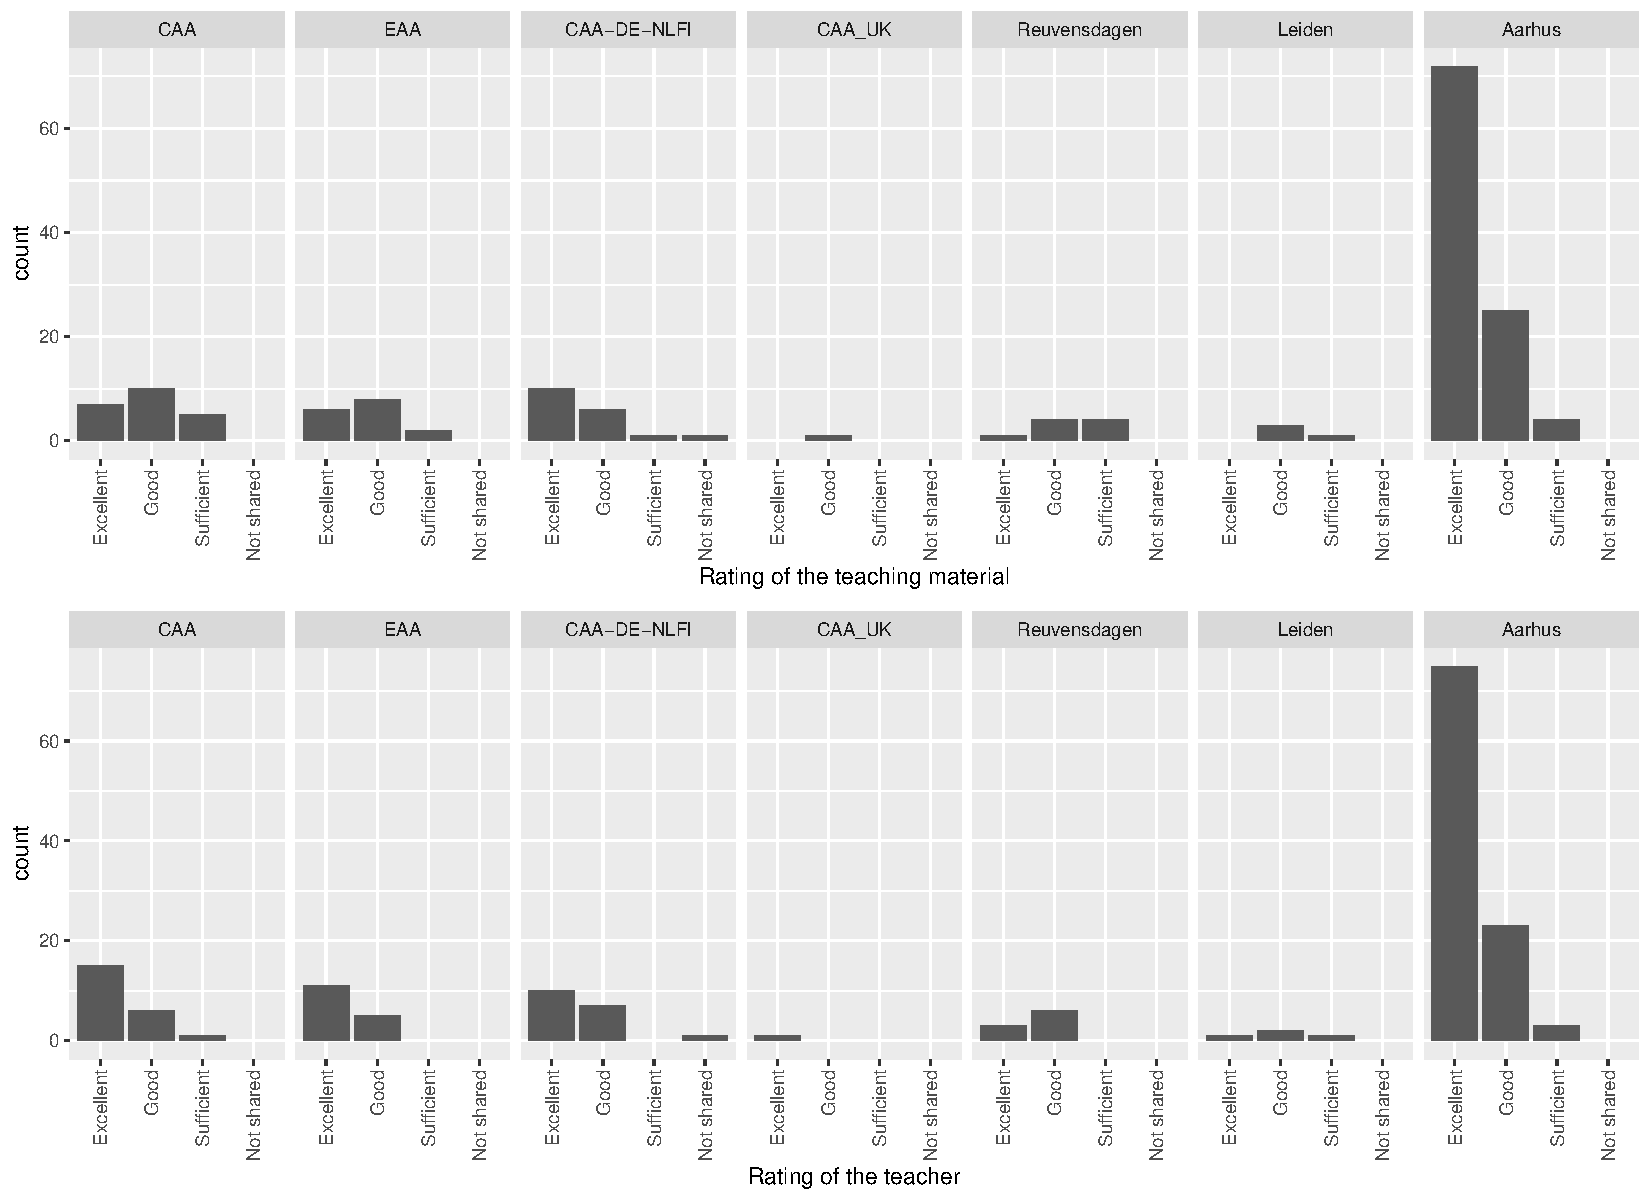
\includegraphics[height=0.5\textheight]{paper_files/figure-latex/rating-teaching-1} 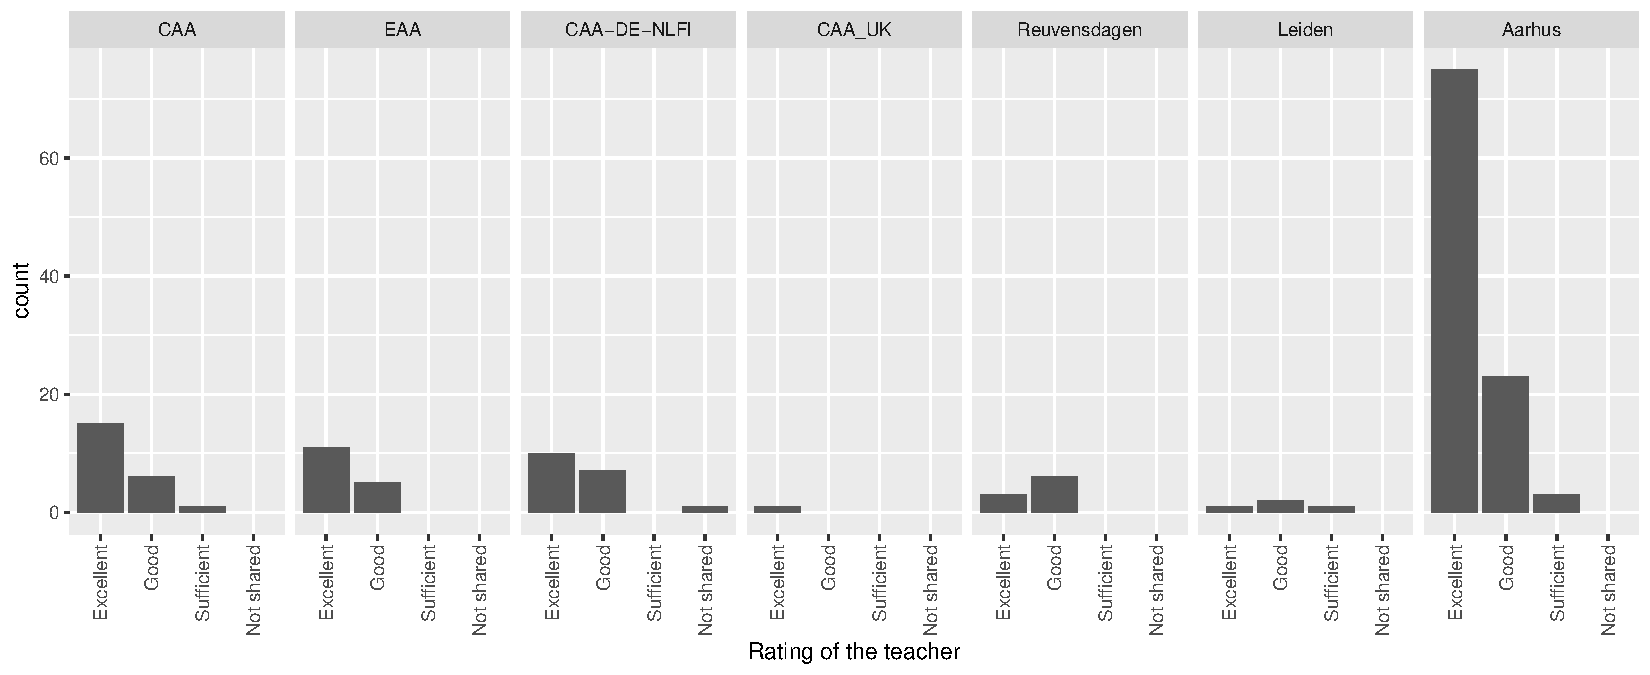
\includegraphics[height=0.5\textheight]{paper_files/figure-latex/rating-teaching-2} \caption{Respondents rating of the teaching material in general faceted for each event.}\label{fig:rating-teaching}
\end{figure}

Two more open questions were asked to the respondents. The first was aimed at learning what aspects the participants liked in the tutorials (What aspects did you like most?), and the other was aimed at getting feedback to improve the tutorials (What would you like to see changed or what could be better/different?).

The respondents generally liked the interactive step-by-step way of going through the tutorials, but also valued the interaction with the teachers strongly. The easy and intuitive introduction into ABM and NetLOGO were also mentioned quite often. This was also observed during the workshops as most participants were working in the own pace and did not need much help. From a didactic point of view, the self-guided and self-paced way of going through the tutorials is very efficient for teachers and limits the frustration of students that may otherwise go too fast or fall behind the class when the tempo is dictated by the teacher.

We also received feedback on possible improvements. During the first workshop, the CAA-conference in Amsterdam in April 2023, we did the first test of the tutorials and we also instructed the participants that this was work in progress. For this and the following few workshops we mostly received feedback about bugs causing the tutorial to crash or creating unexpected behaviour. The number of references to bugs reduced to zero by the end of the project and participants started providing other feedback, for example the wish to see more examples or expanding the tutorials further. Some wanted to introduce more cooperation between participants, which we did not consider primarily aiming the tutorials for individual work. A more cooperative aspect of the education materials is possible, even if harder for online events, and we hope that a wider classroom use of the ABMA materials may deliver solutions. It was also interesting to note that over time more and more people did not see any additional room for improvement indicating that the level, content and format of the tutorials met their needs.

We also asked the participants about their intentions in terms of ABM and their professional life. The majority of the respondents - 88\%, wanted to apply ABM in the future in their research. Some of the respondents were already using ABM in their work. A large group (around 20-30\%) was not sure yet how to apply ABM and wanted to read more on the subject or play a bit with the possibilities. Many respondents also shared the context to which they were thinking to apply ABM mentioning topics such as movement of people or goods over land or water, sometimes in relation to trade or other distribution mechanisms. Others thought of demography, social networks, migration or settlement distributions patterns. The natural environment and the interaction with humans in the past was also mentioned frequently, often in relation to GIS and the question of how complimentary these two computational techniques are. The archaeological periods that the participants were interested in were very diverse, ranging from the Paleolithic to the Medieval period.

\hypertarget{integration-with-learning-and-skills-tracking-frameworks}{%
\subsection{Integration with Learning and Skills Tracking Frameworks}\label{integration-with-learning-and-skills-tracking-frameworks}}

Beyond the creation of the OERs the project also worked on aligning the learning outcomes of the OERs with the Digital Competence Framework for Citizens and the Digital Archaeological Skills Passport.

\hypertarget{the-digital-competence-framework-for-citizens-2.2}{%
\subsubsection{The Digital Competence Framework for Citizens (2.2)}\label{the-digital-competence-framework-for-citizens-2.2}}

As mentioned above, the following competence area's were identified as relevant for the tutorials: 1. Information and data literacy, 2. Communication and collaboration, 3. Digital content creation and, 5. Problem solving (European Commission, Joint Research Centre et al. 2022). In these competence area's various competences are developed towards an advanced or even specialised level. A more extensive description of the Digital Competence Framework for Citizens in relation to Agent-Based Modelling for archaeologists is also available (Visser et al. 2024).

For competence area 1. Information and data literacy: the tutorials mainly address 1.2 Evaluating Data, Information And Digital Content and 1.3 Managing Data, Information And Digital Content. In the ABMA educational materials, users learn about working with data, being critical of their digital content and how to model and manage the data in the context of an ABM. For tutorial 2 the user is expected to be able to find information using the NetLogo(Web) dictionary (\url{http://ccl.northwestern.edu/netlogo/bind/} or \url{http://ccl.northwestern.edu/netlogo/docs/dictionary.html}).

For Competence Area 2. Communication and collaboration the tutorials mainly address 2.1 Interacting Through Digital Technologies, because the users are constantly interacting with digital technologies, but communication is not relevant for the tutorials. However, during the workshops given in the course of the project, participants interacted with each other and the teachers.

Competence Area 3. Digital content creation is one of the main competence areas for the ABM-teaching material. In the process of learning ABM the users are constantly 3.1 Developing Digital Content and 3.2 Integrating And Re-Elaborating Digital Content. The material does not touch upon 3.3 Copyright And Licences, as they fall out of the scope of this project. A very important aspect of learning ABM is 3.4 Programming. The users are guidend through the process of developing the necessary programming skills to build a simulation. While the programming language used - NetLogo - is specific to ABM, its syntax follow general programming patterns and the learning is thus transferable to other programming languages. The users are expected to learn both syntax and more general computational concepts such as modular code development, testing and documenting code.

Competence Area 5. Problem solving is very important and is closely tied to 3.4 Programming, since programming involves a lot of problem solving but also the general principles of model development that have a prominent place in the educational materials. In addition, the creation of a highly complex ABM consists of problem solving all the time, including development of research questions, conceptualisation of theories, experiment design and validating against data - all of which require creative abilities and high level understanding of the scientific process. All competencies are addressed: 5.1 Solving Technical Problems, is common when writing code, learning about coding, error handling and going from pseudocode to real code. The competence 5.2 Identifying Needs And Technological Responses, is a central issue of the course, while 5.3 Creatively Using Digital Technology is an important aspect of so-called model thinking necessary to develop robust and insightful models. In tutorial 2 various aspects of 5.4 Identifying Digital Competence Gaps, are relevant, since this tutorial force the user to assess their knowledge and skills.

\hypertarget{digital-skills-passport}{%
\subsubsection{Digital Skills Passport}\label{digital-skills-passport}}

An archaeological skills passport is a tool for tracking and verifying the archaeological skills that an individual has. The first passport was created as part of \emph{The Ardnamurchan Transitions Project}, a long running investigation of the archaeology and history of the Ardnamurchan Peninsula, Western Scotland, run by the Universities of Leicester and Manchester, with Archaeology Scotland (Cobb and Croucher 2020). Since then the passport has spread around the world to countries such as Germany (Karl et al. 2019) and the United States.~While there are many different versions, in its simplest form it is a log booklet listing skills that others can verify by signing off on their level of competencies.~

A digital skills passport is the same concept as a physical skills passport but it is digitised to overcome some of the drawbacks of a physical skills passport:

\begin{itemize}
\item
  losing a copy means losing a record;
\item
  inability to easily share the log;
\item
  costs of production;
\item
  ability to verify those signing off on skill levels.~
\end{itemize}

A trans-Atlantic consortium has been established to create a digital archaeological skills passport. It consists of the professional body in the United States of America, the \emph{Register of Professional Archaeologists} and five archaeological companies in Europe, working and based in Ireland, the United Kingdom, the Netherlands, Germany and France. This is the passport that the ABMA integrate the OERs with.~

Agent Based Modelling (ABM) will be placed within the transferable skills category of the Digital Archaeological Skills Passport. This will be facilitated by the creation of a larger category of Analytical Skills and then a sub-category of modelling:

\begin{verbatim}
38  Analytical Skills
  38.1 Modelling
      38.1.1 Computational Modelling
        38.1.1.1 Agent Based Modelling
          38.1.1.1.1 Software mastery
            38.1.1.1.1.1 Creation of models and understanding of key components
             38.1.1.1.1.2 Integration of other fields - GIS, network science
          38.1.1.1.2 Analysis and interpretation of results
     38.1.2 Mathematical Modelling
etc.
\end{verbatim}

The digital skills passport has not launched yet, but when it is, it will be found at this url: \url{https://archaeologypassport.com}.

\hypertarget{dissemination-of-tutorials}{%
\subsection{Dissemination of tutorials}\label{dissemination-of-tutorials}}

The tutorials are publicly hosted on GitHub (\url{https://github.com/ABMArchaeologists/ABMA_tutorials/}) and are citeable (Rocks-Macqueen et al. 2024). Anyone interested can download the tutorials and their source code. To increase the accessibility and visibility of the tutorials, they are also hosted on a static website (\href{https://ABMArchaeologists.github.io/ABMA_Website/\#/}{https://ABMArchaeologists.github.io/ABMA\_Website}) can be followed without the need to download any software. The source code of the website is also openly available (Jutte et al. 2024).

Besides, the tutorial, the website provides: a link that can be used for feedback, basic explanations of agent-based modelling, an introductory presentation from one of the workshops, videos from an online course at Leiden University (Scherjon, Romanowska and Lambers 2019) and external resources people can use to learn agent-based modelling. The website was mainly developed by a student group from Saxion University of Applied Sciences, see the acknowledgements.

\hypertarget{conclusion}{%
\section{Conclusion}\label{conclusion}}

The process of creating and testing Open Educational Resources for Agent-Based Modelling for Archaeologists showed us many things. The demand for tutorials exceeded our expectations, showing the importance of creating these materials. The testing of tutorials during workshops at international an national conferences proved very useful in gaining direct feedback. This greatly helped improving the material. The tutorials have proven their use in guiding learners into understanding ABM in an archaeological context. The international cooperation improved the quality of the material and also the accessibility of the material for various audiences. The integration in the Digital competency framework and Skills passport increased the didactic and pedagogic quality even while the latter is not yet published.

Future aspects of these open learning materials will be the further application and integration within the educational programmes in our universities and hopefully in others too. We have made the material openly available and we hope that the ABM-community will stay involved and that future updates will be community driven.

\hypertarget{acknowledgements}{%
\section{Acknowledgements}\label{acknowledgements}}

This project was undertaken with the support of the Erasmus+ programme of the European Union (\url{https://erasmus-plus.ec.europa.eu/nl/projects/search/details/2021-2-IE01-KA220-VET-000049054}).

We would like to thank the student groups at Saxion University of Applied Sciences that worked with us:

\begin{itemize}
\item
  September 2022-February 2023: Dany Dragoi, Liam van den Bosch, Marko Stojkovic, Max van Duinen, Nora van den Engel, Roan Man, Stefan Oostingh and their tutor: Mark Spanjer.
\item
  February 2022-July 2023: Alice Overgaauw, Johan Broersma, Mandy Hazenberg, Paulina Fulneczek, Ties Heesink and their tutor: Jan Willem Huson.
\item
  September 2023-February 2024: Arnfinn Sijbrant, Eva Baan, Jip Mulder, Robert Aalpoel, Sem Lucas, Sterre Regts and their tutor: Jan Willem Huson.
\end{itemize}

This last group, we want to thank for providing us with the website on which the tutorials are hosted.

We had help from many people during the various workshops and we would like to thank them for their help (in alphabetical order of their first name): Adéla Sobotkova, Agnes Schneider, Alice Poorthuis, Eduardo Herrera Malatesta, Jens Emil Bødstrup Christoffersen, Johan Broersma, Magnus Lindholm Nielsen, Mandy Hazenberg, María Coto Sarmiento, Paulina Fulneczek, Petra Hermankova, Ties Heesink. We also want to thank all the participants of our workshops.

Funding acknowledgements: the publication was financed by The Carlsberg Foundation's \emph{Young Researcher Fellowship} (CF21-0382); IR was supported by the European Union's Horizon 2020 Research and Innovation Programme under the Marie Skłodowska-Curie grant agreement no 754513, the Aarhus University Research Foundation and FWO grant number W001220N.

\hypertarget{references}{%
\section*{References}\label{references}}
\addcontentsline{toc}{section}{References}

\hypertarget{refs}{}
\begin{CSLReferences}{1}{0}
\leavevmode\vadjust pre{\hypertarget{ref-aalpoel2024}{}}%
Aalpoel, R, Baan, E, Lucas, S, Mulder, J, Regts, S, Sijbrant, A, Jutte, A and Visser, R. 2024 \emph{Teaching material Agent-Based Modelling for Archaeologists (EN/NL)} DOI: https://doi.org/\href{https://doi.org/10.5281/zenodo.10950153}{10.5281/zenodo.10950153}.

\leavevmode\vadjust pre{\hypertarget{ref-cobb2020}{}}%
Cobb, H and Croucher, K. 2020 \emph{Pedagogy, political economy, and training}. In: Cobb, H and Croucher, K (eds.). Oxford University Press. p. 0. DOI: https://doi.org/\href{https://doi.org/10.1093/oso/9780198784258.003.0004}{10.1093/oso/9780198784258.003.0004}.

\leavevmode\vadjust pre{\hypertarget{ref-councilofeurope2020}{}}%
Council of Europe. 2020. \emph{\href{http://www.coe.int/lang-cefr}{Common european framework of reference for languages: Learning, teaching, assessment. Companion volume}}. Strasbourg: Council of Europe Publishing.

\leavevmode\vadjust pre{\hypertarget{ref-davies2018}{}}%
Davies, B and Romanowska, I. 2018 An emergent community? Agent-based modelers in archaeology. \emph{The SAA Archaeological Record} 18(2): 27--32.

\leavevmode\vadjust pre{\hypertarget{ref-epstein1996}{}}%
Epstein, JM and Axtell, RL. 1996. \emph{Growing Artificial Societies: Social Science from the Bottom Up}. The MIT Press. DOI: https://doi.org/\href{https://doi.org/10.7551/mitpress/3374.001.0001}{10.7551/mitpress/3374.001.0001}.

\leavevmode\vadjust pre{\hypertarget{ref-europeancommissionjointresearchcentre2022}{}}%
European Commission, Joint Research Centre, Vuorikari, R, Kluzer, S and Punie, Y. 2022. \emph{\href{https://data.europa.eu/doi/10.2760/115376}{DigComp 2.2: The Digital Competence Framework for Citizens - With new examples of knowledge, skills and attitudes}}.

\leavevmode\vadjust pre{\hypertarget{ref-grolemund2011}{}}%
Grolemund, G and Wickham, H. 2011 \href{https://www.jstatsoft.org/v40/i03/}{Dates and times made easy with lubridate}. \emph{Journal of Statistical Software} 40(3): 125.

\leavevmode\vadjust pre{\hypertarget{ref-jutte2024}{}}%
Jutte, A, Aalpoel, R, Baan, E, Regts, S, Lucas, S, Mulder, J, Sijbrant, A, Visser, RM, Rocks-Macqueen, D, Knaap, L van der, Romanowska, I, Brughmans, T, Lambers, K and Aitchison, K. 2024. \emph{Agent based modelling for archaeologists: Website source}. Zenodo. DOI: https://doi.org/\href{https://doi.org/10.5281/zenodo.10931759}{10.5281/zenodo.10931759}.

\leavevmode\vadjust pre{\hypertarget{ref-karl2019}{}}%
Karl, R, Möller, K, Connolly, D, Trausmuth, T, Krierer, KR, Rocks-Macqueen, D, Aitchison, K, Edeso, M, Pintucci, A and Marciniak, A. 2019 Der archäologische Grabungs-Kompetenz-Pass {\textendash} ein Mittel zur Dokumentation durch Praxis erworbener archäologischer Fertigkeiten. \emph{Archäologische Informationen} 42: 237--249. DOI: https://doi.org/\href{https://doi.org/10.11588/ai.2019.0.69362}{10.11588/ai.2019.0.69362}.

\leavevmode\vadjust pre{\hypertarget{ref-marwick2017}{}}%
Marwick, B. 2017 Computational Reproducibility in Archaeological Research: Basic Principles and a Case Study of Their Implementation. \emph{Journal of Archaeological Method and Theory} 24(2): 424--450. DOI: https://doi.org/\href{https://doi.org/10.1007/s10816-015-9272-9}{10.1007/s10816-015-9272-9}.

\leavevmode\vadjust pre{\hypertarget{ref-rcoreteam2023}{}}%
R Core Team. 2023 \emph{\href{https://www.R-project.org/}{R: A language and environment for statistical computing}}.

\leavevmode\vadjust pre{\hypertarget{ref-rocks-macqueen2024}{}}%
Rocks-Macqueen, D, Knaap, L van der, Romanowska, I, Jutte, A, Visser, RM, Brughmans, T, Lambers, K and Aitchison, K. 2024. \emph{Agent based modelling for archaeologists: tutorials}. Zenodo. DOI: https://doi.org/\href{https://doi.org/10.5281/zenodo.10931587}{10.5281/zenodo.10931587}.

\leavevmode\vadjust pre{\hypertarget{ref-romanowska2018}{}}%
Romanowska, I. 2018 \emph{Using agent-based modelling to infer economic processes in the past}. In: Remesal Rodriguez, J, Revilla Calvo, V, and Bermudez Lorenzo, JM (eds.). Barcelona, Spain: Universitat de Barcelona * Servei de Publicacions. pp. 107--118.

\leavevmode\vadjust pre{\hypertarget{ref-romanowska2023}{}}%
Romanowska, I and Scherjon, F. 2023 \emph{Bibliometric analysis of agent-based simulation in archaeology: People, topics, and future prospects}. In: Kalayci, T, Lambers, K, and Klinkenberg, V (eds.). Analecta praehistorica leidensia. Leiden: Sidestone Press. pp. 95--112. DOI: https://doi.org/\href{https://doi.org/10.59641/f48820ir}{10.59641/f48820ir}.

\leavevmode\vadjust pre{\hypertarget{ref-romanowska2021a}{}}%
Romanowska, I, Wren, CD and Crabtree, SA. 2021. \emph{\href{https://www.sfipress.org/books/agent-based-modeling-archaeology}{Agent-based modeling for archaeology: Simulating the complexity of societies}}. Santa Fe: Santa Fe Institute Press.

\leavevmode\vadjust pre{\hypertarget{ref-scherjon2019}{}}%
Scherjon, F, Romanowska, I and Lambers, K. 2019 Digitally Teaching Digital Skills: Lessons Drawn from a Small Private Online Course (SPOC) on {`}Modelling and Simulation in Archaeology{'} at Leiden University. \emph{Journal of Computer Applications in Archaeology} 2(1): 7988. DOI: https://doi.org/\href{https://doi.org/10.5334/jcaa.26}{10.5334/jcaa.26}.

\leavevmode\vadjust pre{\hypertarget{ref-visser2024}{}}%
Visser, R, Lambers, K, Aitchison, K, Jutte, A, Rocks-Macqueen, D, Knaap, L van der, Romanowska, I and Brughmans, T. 2024 \emph{The Digital Competence Framework for Citizens (2.2) and Agent-Based modelling for Archaeologists}. DOI: https://doi.org/\href{https://doi.org/10.5281/zenodo.11046488}{10.5281/zenodo.11046488}.

\leavevmode\vadjust pre{\hypertarget{ref-wickham2016}{}}%
Wickham, H. 2016. \emph{\href{http://ggplot2.org}{ggplot2: Elegant graphics for data analysis}}. Springer-Verlag New York.

\leavevmode\vadjust pre{\hypertarget{ref-wickham2023b}{}}%
Wickham, H. 2023a \emph{\href{https://forcats.tidyverse.org/}{Forcats: Tools for working with categorical variables (factors)}}.

\leavevmode\vadjust pre{\hypertarget{ref-wickham2023c}{}}%
Wickham, H. 2023b \emph{\href{https://stringr.tidyverse.org}{Stringr: Simple, consistent wrappers for common string operations}}.

\leavevmode\vadjust pre{\hypertarget{ref-wickham2023a}{}}%
Wickham, H, François, R, Henry, L, Müller, K and Vaughan, D. 2023 \emph{\href{https://dplyr.tidyverse.org}{Dplyr: A grammar of data manipulation}}.

\leavevmode\vadjust pre{\hypertarget{ref-wickham2023}{}}%
Wickham, H, Vaughan, D and Girlich, M. 2023 \emph{\href{https://tidyr.tidyverse.org}{Tidyr: Tidy messy data}}.

\leavevmode\vadjust pre{\hypertarget{ref-young1995}{}}%
Young, DA and Bettinger, RL. 1995 Simulating the global human expansion in the late pleistocene. \emph{Journal of Archaeological Science} 22(1): 89--92. DOI: https://doi.org/\href{https://doi.org/10.1016/S0305-4403(95)80165-0}{10.1016/S0305-4403(95)80165-0}.

\end{CSLReferences}

\end{document}
